\subsubsection{Micro Architecture}

Distributed ledger technology is at the very core of any decentralised project. In this project, it provides the compute backbone, the only non-local, stateful system in the project architecture. Whilst this compute backbone has, until now, been observed as a monolithic module, we now consider it's implementation and own micro-architecture.

It is trivial that every identity, every user of the proposed system, needs to have their own state representative of files they own and associated metadata. It is also trivial that every group that exists on the network must exist as a collection of identities and this should exist as some state along with associated metadata. We therefore need two contracts, as a minimum, each representative of some state. These will be called the 'Storage' contract and the 'Group' contract.

However, these two contracts will be instantiated in arbitrary sizes. Upon launch of a system, there would be zero of either, but contract instantiation is expected to follow user adoption. Since this is a decentralised application, a static reference is required to the root of the project's compute such that it can always be found. In a production environment this might be represented by a versioning contract which would hold the contract address of a root contract against a version number, an example contract can be found in Program Code \ref{code:ethereum_versioning} (Appendix). For a proof of concept this versioning contract is unnecessary. 

\paragraph{Storage Contract}

\paragraph{Group Contract}

\paragraph{Registry Contract}

% TODO: Get to the below diagram

\begin{figure}[H]
  \centering
  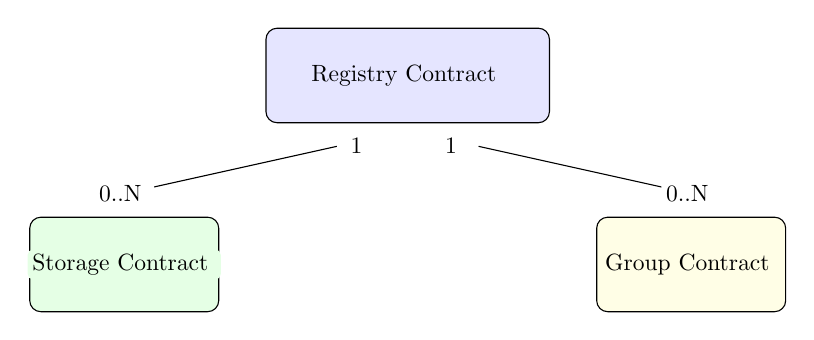
\begin{tikzpicture}[scale = 0.6, every node/.style={scale = 0.85}, every node/.append style={fill = white, rounded corners = 2pt, inner sep = 2pt, align = center}]

  \draw [rounded corners, fill=blue!10] (-3, 2) rectangle (3, 0);
  \node [fill=blue!10] at (0, 1) { Registry Contract };

  \draw [rounded corners, fill=green!10] (-8, -4) rectangle (-4, -2);
  \node [fill=green!10] at (-6, -3) { Storage Contract };

  \draw [rounded corners, fill=yellow!10] (4, -4) rectangle (8, -2);
  \node [fill=yellow!10] at (6, -3) { Group Contract };

  \draw (-1.5,  -0.5) -- (-6,  -1.5);
  \node at (-1, -0.5) { 1 };
  \node at (-6, -1.5) { 0..N };

  \draw (1.5,  -0.5) -- (6,  -1.5);
  \node at (1, -0.5) { 1 };
  \node at (6, -1.5) { 0..N };

  \end{tikzpicture} \\
  \caption{
  	Ethereum Micro-Architecture
  }{
    Outline of the micro-architecture of Ethereum contracts, shown with cardinality.
  }
  \label{fig:ethereum_micro_architecture}
\end{figure}


Figure \ref{fig:ethereum_micro_architecture}
